\documentclass[12pt]{article}
\linespread{1.25}
\usepackage{times}

\usepackage{pgfplots}
\pgfplotsset{compat = newest}
\usetikzlibrary{positioning, arrows.meta}
\usepgfplotslibrary{fillbetween}
\usepackage{amsmath}

\begin{document}

\begin{center}
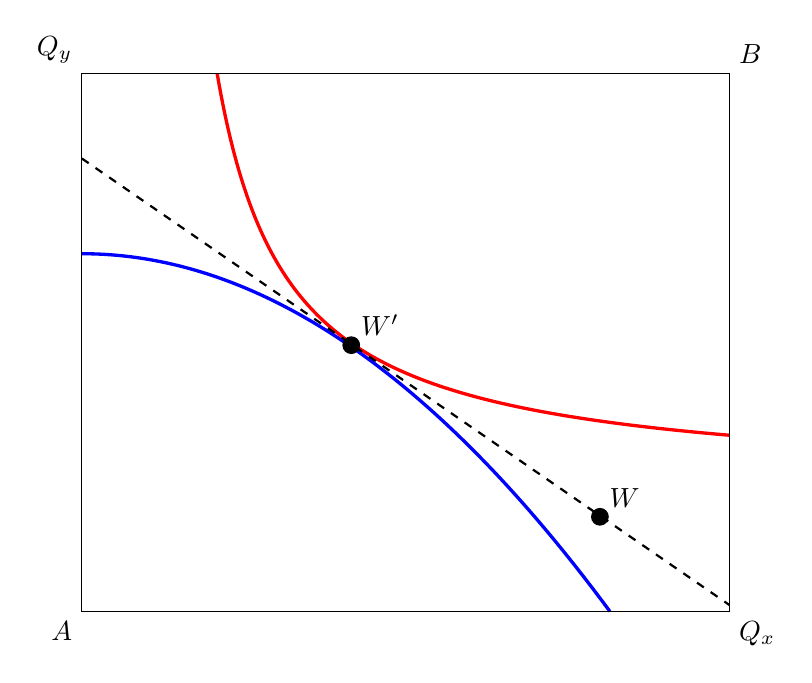
\begin{tikzpicture}
\begin{axis}[
scale = 1.2,
xmin = 0, xmax = 10,
ymin = 0, ymax = 10,
axis lines* = box,
xtick = \empty, ytick = \empty,
axis on top,
clip = false,
]
% Curves and lines
\addplot [domain = 0:10, restrict y to domain = 0:10, samples = 5000, color = red, very thick]{25/(3*x-3)+2.35};
\addplot [domain = 0:10, restrict y to domain = 0:10, samples = 5000, color = blue, very thick]{6.65-0.1*x^2};
\addplot [domain = 0:10, restrict y to domain = 0:10, samples = 5000, color = black, dashed, thick]{-0.83*x+8.42};

% Coordinate points
\addplot[color=black, mark=*, only marks, mark size=3pt] coordinates {(4.16, 4.95) (8, 1.76)};

% Labels
\node [below left] at (0, 0) {$A$};
\node [above right] at (10, 10) {$B$};
\node [below right] at (10, 0) {$Q_x$};
\node [above left] at (0, 10) {$Q_y$};
\node [above right] at (8, 1.76) {$W$};
\node [above right] at (4.16, 4.95) {$W^\prime$};
\end{axis}
\end{tikzpicture}
\end{center}
\textbf{Figure 9-3:} The market equilibrium, $W^\prime$, in an Edgeworth box between two consumers, $A$ and $B$, and two commodities, $x$ and $y$.

\end{document}
